\chapter{روش انجام پروژه}
\section{مقدمه}

برای اجرای این پروژه راه‌های متفاوتی مورد بررسی قرار داده شد تا بتوان بهترین آنها را روی پهپاد پیاده‌سازی کرد. نتیجه نهایی پیاده سازی ۳ شبکه کانولوشن
به صورت پی در پی است. شبکه اول برای آشکارسازی موقعیت کف دست است. بدین صورت که هر فریم گرفته‌شده از دوربین پهپاد 
پس از تغییر اندازه به یک ماتریس ددد*پپپپ*۳ به ورودی مدل داده می‌شود و پس از پردازش آن خروجی یک ماتریس ۲۵۶*۲۵۶*۳ است که جعبه محدودکننده 
دست را شامل می‌شود. پس از آن، این ماتریس به مدل دوم به عنوان ورودی داده می‌شود، در این مدل جعبه مرزی برش خورده دست به صورت یک ماتریس گرفته‌شده و خروجی آن برابر ۲۱ نقطه 
سه بعدی عطف دست و شاخص دست(راست یا چپ) است.  در ادامه مدل سوم به عنوان ورودی، یک ماتریس ۲۱*۲ می‌گیرد که مختصات نقاط  طول و عرض هر نقطه عطف دست است س=
چرا که عمق تصویر با توجه به ژست‌های در نظر گرفته شده از اهمیت بالایی برخوردار نیست. و در خروجی پیش‌بینی می‌کند که کدام ژست دست مد نظر کاربر است. با توجه به این پروژه ۹ ژست 
گوناگون مدنظر قرار گرفته‌شده (کاربر می‌تواند ژست‌های جدیدی اضافه کند)، خروجی شبکه کانولوشن شامل ۱۰ کلاس 
کلاس است که ۹ کلاس برای ژست‌ها و کلاسی برای زمانی که هیچ کدام از ژست‌ها انتخاب نشده در نظر گرفته‌شده.


\section{دیتاست}

\begin{figure}[h]
    \centering
    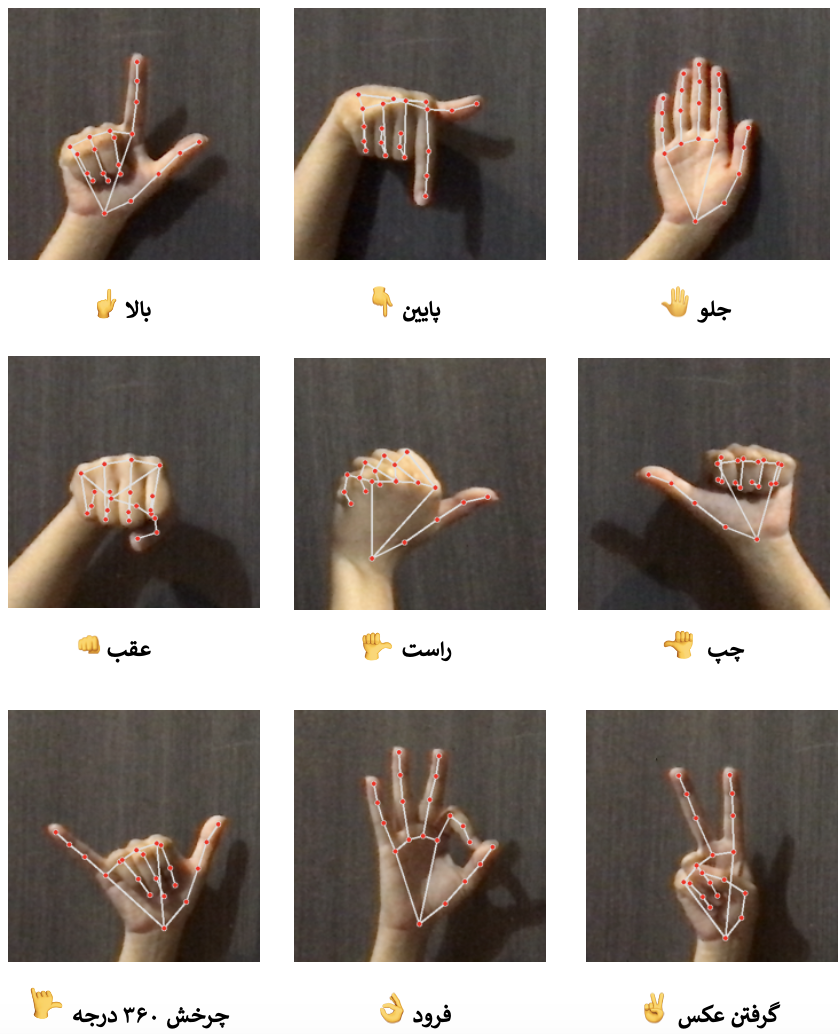
\includegraphics[width=0.7\textwidth]{gestures.png}
    \caption{نمونه‌ای از ژست‌های انتخاب‌شده در مجموعه داده‌ها}
\end{figure}




\section{اهمیت ژست دست}
وقتی مردم صحبت می کنند، ژست می گیرند. ژست جزء اساسی زبان است که اطلاعات معنادار و منحصر به فردی را انتقال می‌دهد. ژست‌ها به گوینده کمک می‌کنند تا اهداف خود را بهتر منعکس کند. 
آن‌‌ها نقش های بسیاری را در ارتباط، یادگیری و درک هم برای افرادی که آنها را مشاهده می کنند و هم برای کسانی که آنها را ایجاد می کنند، ایفا می کنند.
وقتی مردم صحبت می کنند، دستان خود را حرکت می دهند. به حرکات خود به خودی دست که در ریتم گفتار ایجاد می شوند، حرکات هم گفتاری \LTRfootnote{co-speech gestures}
نامیده می شوند و مردم از همه فرهنگ ها و پیشینه های زبانی شناخته شده ژست می گیرند و برای ارتباط از حرکات هم گفتاری برای رساندن بهتر مفهوم خود کمک می‌گیرند.
در واقع، نوزادان قبل از اینکه اولین کلمات خود را بیان کنند، از انواع ژست‌ها استفاده می‌کنند. دست‌های ما به ما کمک می‌کنند صحبت کنیم، فکر کنیم، و به خاطر بسپاریم، گاهی دانش
منحصر به فردی را که هنوز نمی‌توان به زبان آورد، آشکار می‌کنند. به طوری که می‌توان گفت ژست‌ها اغلب به عنوان زبان گفتاری ثانویه در نظر گرفته می شود.\cite{clough2020role}
ژست‌ها به‌ویژه زمانی مؤثر هستند که مزیتی نسبت به کلمات داشته باشند. \cite{kang2016hands}
توانایی درک شکل و حرکت دست‌ها می‌تواند یک جزء حیاتی در بهبود تجربه کاربر \LTRfootnote{user experience} 
در حوزه‌ها و پلتفرم‌های مختلف فناوری باشد. درک مفهوم ژست دست در زمان واقعی برای افراد به طور طبیعی وجود دارد، یک کار بینایی 
کامپیوتری کاملاً چالش برانگیز است، زیرا دست ها اغلب خود یا یکدیگر را مسدود می کنند مانند انسداد انگشت، کف دست و لرزش دست و فاقد الگوهای کنتراست بالا هستند.\cite{zhang2020mediapipe}

\section{کنترل پهپاد}
اکثر پهپادهای تجاری موجود در بازار یا دارای کنترلرهای طراحی شده ویژه هستند، یا دارای فرستنده سیگنال اختصاصی و برنامه‌های نرم‌افزاری هستند که روی دستگاه‌های دستی کاربران 
مانند تلفن‌های همراه یا تبلت‌ها اجرا می‌شوند. در هر دو مورد، کنترل‌کننده فرمان‌هایی را با اطلاعات دقیق از طریق کانال‌های بی‌سیم مانند 
وای‌فای یا بلوتوث ارسال می‌کند. اخیراً محصولات تجاری وجود داشته است که حرکات دست را به عنوان یک مکانیسم کنترل قابل اجرا معرفی می کنند. برای گرفتن ژست ها، دو رویکرد وجود دارد.
\begin{itemize}
    \item	استفاده از دستکش های طراحی شده ویژه: کنترل کننده بر روی دستکشی که توسط کاربران استفاده می شود نصب می شود و در زمان واقعی انحراف، گام و چرخش دست را شناسایی می کند 
    تا به حرکات مربوطه برای پهپاد را شناسایی و ارسال کند. محصولات عبارتند از \lr{Kd Interactive Aura Drone} و \lr{MenKind Motion Control Drone}
    \item 	استفاده از بینایی کامپیوتر از طریق دوربین: این دستگاه‌ها از دوربین نصب شده روی پهپاد استفاده می‌کنند تا بتوانند در لحظه تشخیص دهند که دست کاربر کجاست
    و در چه حالتی قرار دارد تا پهپاد را کنترل کند. محصولات عبارتند از \lr{DJI Spark Drone} 
\end{itemize}



\section{ابزار ها و نرم افزار های مورد استفاده}
\subsection{\lr{TensorFlow}}
\lr{TensorFlow} یک کتابخانه نرم افزاری رایگان و منبع باز برای یادگیری ماشین و هوش مصنوعی است. می توان از آن در طیف وسیعی از وظایف استفاده کرد، اما تمرکز ویژه ای بر آموزش و استنتاج شبکه های عصبی عمیق دارد.

\subsection{\lr{MediaPipe}}
\lr{MediaPipe} مجموعه ای از کتابخانه ها و ابزارهایی است که از تکنیک‌های هوش مصنوعی و یادگیری ماشین در برنامه‌های خود استفاده می‌کند.
این کتابخانه برای برنامه‌نویسان یادگیری ماشین از جمله محققان، دانشجویان و توسعه‌دهندگان نرم‌افزار، که برنامه‌های کاربردی یادگیری ماشین را پیاده‌سازی می‌کنند، نمونه‌های
اولیه فناوری را طراحی می‌کند تا بتوان پروژه‌ها را تا حد امکان ساده کرد.
برنامه‌هایی که داده‌های حسی مثل ویدیو و صدا را با نرخ فریم بالا پردازش می‌کند تا تجربه کاربر را بهتر کند. مراحل پردازش یا مدل‌های استنتاجی ممکن است دشوار باشد، چون 
گاهی اتصال بین مراحل زیاد است. همچنین، توسعه برنامه برای پلتفرم‌ زمان‌بر است. \cite{lugaresi2019mediapipe}
\\
\lr{Media Pipe} این چالش‌ها را با انتزاع و اتصال مدل‌های مختلف به یکدیگر در یک چارچوب مناسب حل می‌کند. با استفاده از \lr{MediaPipe}، می‌توان یک لوله پردازش را به صورت 
گراف از اجزای مختلف، از جمله مدل‌های استنتاجی و عملکردهای پردازش رسانه‌ای، ساخت.
همچنین این کتابخانه می‌تواند مطابق با نیازهای افراد خود سفارشی شود و در پلتفرم‌های مختلف توسعه پیدا کند \cite{harris2021applying}.
\\
در مجموعه \lr{MediaPipe} نیز از کتابخانه‌های مختلفی برای پیاده‌سازی برنامه ها استفاده می‌شود. از جمله آنها می‌توان به \lr{Tensor Flow}، \lr{PyTorch}، \lr{OpenCV}، \lr{CNTK} و \lr{MXNet} اشاره کرد. \cite{harris2021applying}


\section{مدیاپایپ}
برای پیاده سازی شبکه‌های تشخیص کف دست و پیدا کردن نقاط عطف دست از مدل‌های از قبل آموزش دیده\LTRfootnote{Pretrained} کتابخانه مدیاپایپ کمک گرفته‌شده است. مدیاپایپ  از یک خط لوله
یادگیری ماشین متشکل از چندین مدل که با هم کار می کنند استفاده می کند: یک مدل تشخیص کف دست \LTRfootnote{Palm detection model}
که تصویر را از ورودی می‌گیرد و  عکس محدوده دست را به عنوان خروجی دریافت میکند و یک مدل تشخیص نقاط عطف دست \LTRfootnote{Hand landmark model}
که عکس دست را به عنوان ورودی گرفته و مختصات‌ 21 نقطه کلیدی بند‌های انگشتان دست را در ناحیه دست تشخیص می دهد.

\subsection{مدل تشخیص کف دست}
مدل تشخیص کف دست مدیاپایپ دارای دقت متوسط ۷.۹۵ درصد است که این دقت بالا با استفاده از استراتژی‌های مختلف به‌دست آمده است. ابتدا، به جای آشکار کردن دست\LTRfootnote{hand detector}
، آشکار کردن کف دست را به مدل آموزش می‌دهند، زیرا پیدا کردن محدود از اجسام سفت و سخت مانند کف دست و مشت بسیار ساده‌تر از تشخیص دست‌ها با 
انگشتان مفصلی است. علاوه بر این، از آنجایی که کف دست‌ها اشیاء کوچکی هستند، الگوریتم سرکوب غیر حداکثری \LTRfootnote{Non-maximum suppression}
که یک تکنیک پس پردازش \LTRfootnote{post-process} است و در تشخیص اشیا برای حذف تشخیص های تکراری \LTRfootnote{duplicate detections}
و انتخاب مرتبط ترین اشیاء شناسایی شده استفاده می شود. این به کاهش مثبت کاذب \LTRfootnote{false positive} و پیچیدگی محاسباتی \LTRfootnote{computational complexity}
یک الگوریتم تشخیص کمک می کند. تا بهترین محدوده مربعی \LTRfootnote{bounding box} با واریانس بالا \LTRfootnote{high scale variance} را بدست آورد. \cite{zhang2020mediapipe}


\begin{figure}[h]
    \centering
    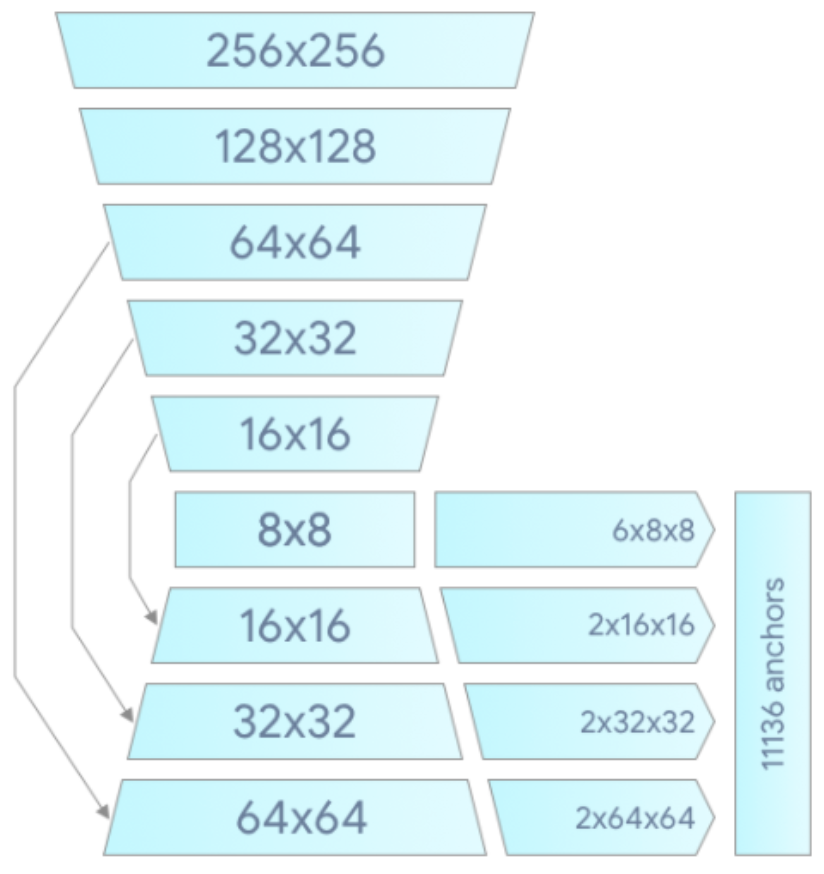
\includegraphics[width=0.4\textwidth]{hand_detector.png}
    \caption{معماری مدل آشکارساز کف دست}
\end{figure}

\begin{figure}[h]
    \centering
    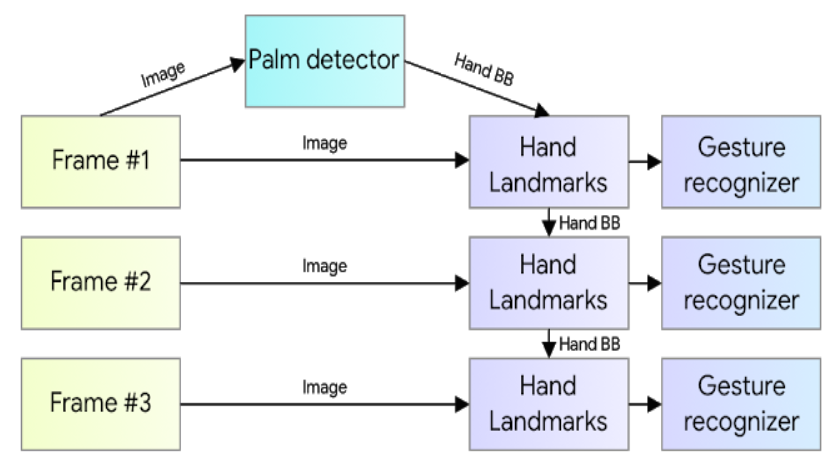
\includegraphics[width=0.7\textwidth]{mediapipe.png}
    \caption{خط لوله تشخیص دست}
\end{figure}

\subsection{مدل تشخیص نقاط عطف دست}
در این مرحله مکان‌یابی مختصات 21 نقطه کلیدی بند‌های انگشتان دست که شامل سه بعد است از طریق رگرسیون \LTRfootnote{regression}
انجام می‌شود. این مدل بر روی 30 هزار تصویر دنیای واقعی با 21 مختصات سه بعدی برچسب زده‌شده \LTRfootnote{labeling}
آموزش دیده‌است .برای پوشش بهتر ژست‌های احتمالی دست و ارائه نظارت بیشتر بر ماهیت هندسه دست، این دیتاست از مدل‌های دست مصنوعی
با کیفیت بالا را نیز روی پس‌زمینه‌های مختلف ارائه می‌کند تا دقت را به بالاترین حد ممکن برساند. این مدل حتی در برابر دست های نیمه نیز عملکرد قوی نشان می‌دهد. \cite{zhang2020mediapipe}

\begin{figure}[h]
    \centering
    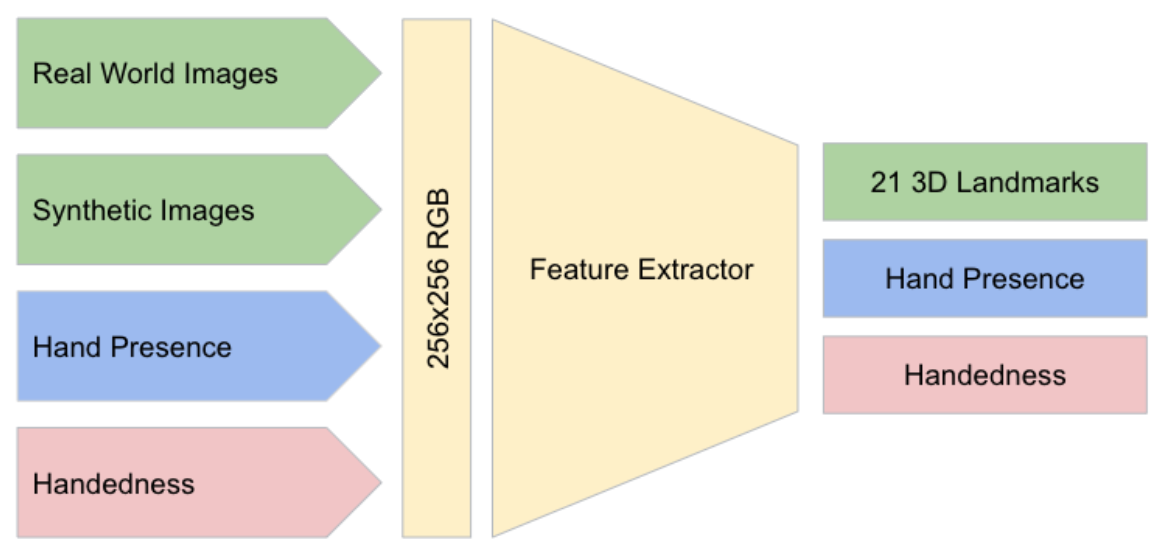
\includegraphics[width=0.7\textwidth]{landmark.png}
    \caption{معماری مدل نقطه عطف دست. این مدل دارای سه خروجی است که یک استخراج کننده ویژگی را به اشتراک می گذارند. هر سر توسط مجموعه داده های مربوطه که با همان رنگ مشخص شده اند آموزش داده می شود.}
\end{figure}

\begin{figure}[h]
    \centering
    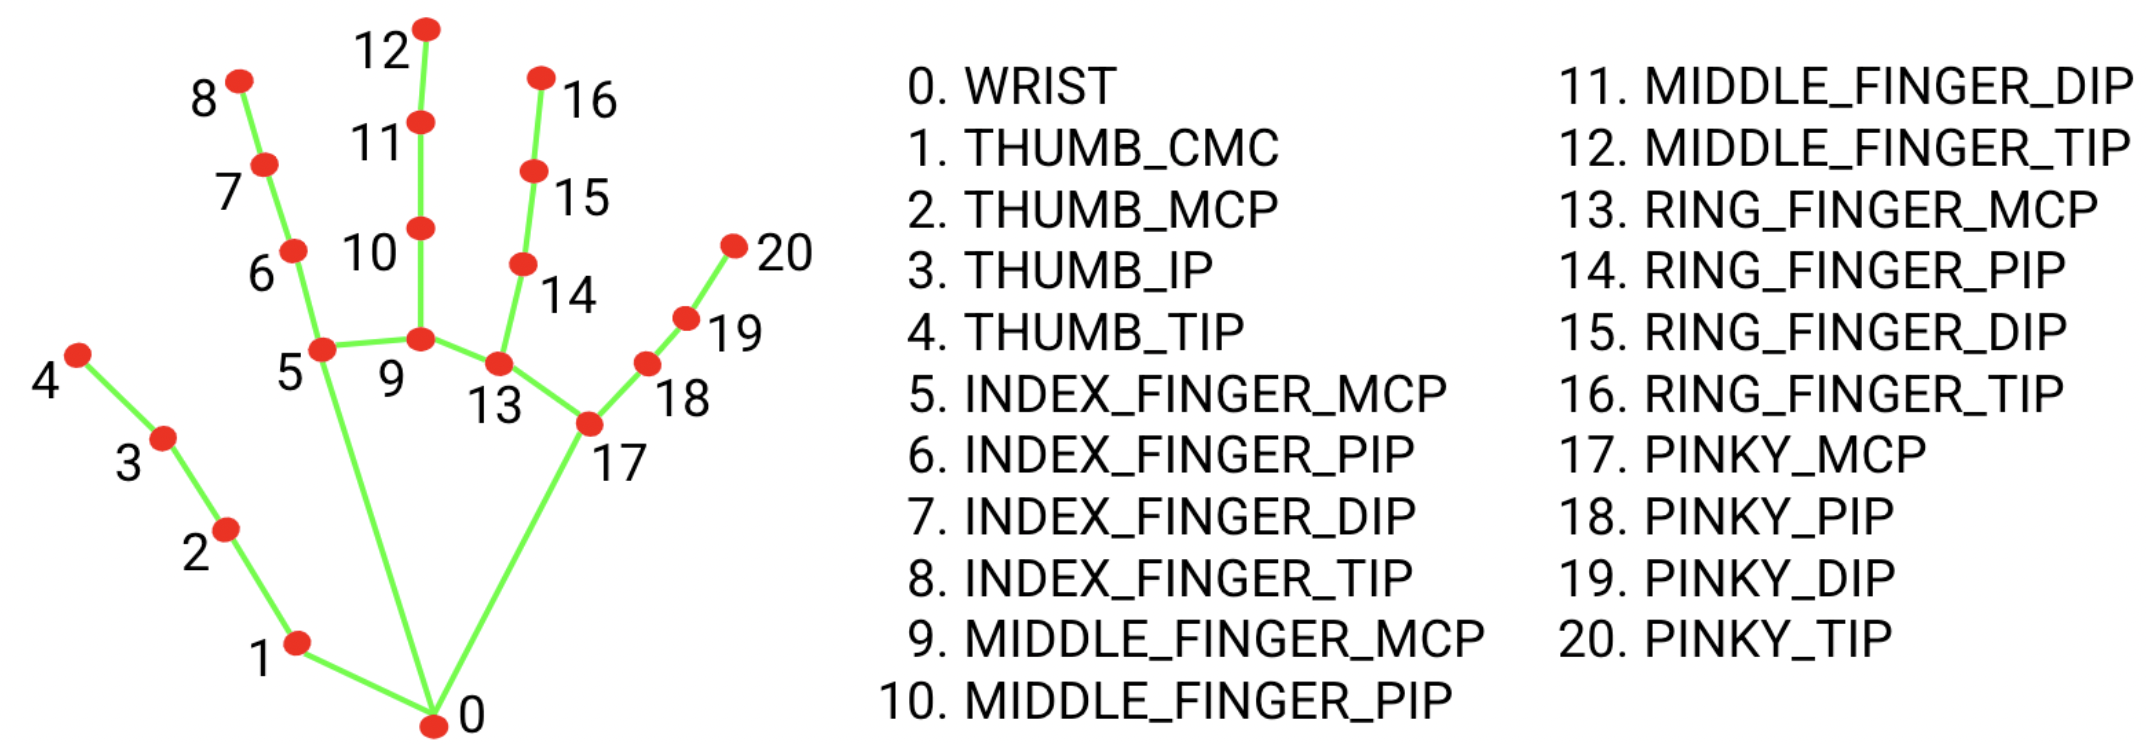
\includegraphics[width=1\textwidth]{hand-landmarks.png}
    \caption{موقعیت ۲۱ نقطه کلیدی در ناحیه دست}
\end{figure}



\section{پیش‌پردازش}
برای ورود نقاط عطف دست به مدل تعیین ژست به ۲۱ مختصات x و y نیاز داریم. خروجی مدل تعیین مختصات نقاط عطف دست برابر مختصات مطلق پیکسل ها نسبت به گوشه سمت 
چپ پایین تصویر است. این نقاط با توجه به اندازه عکس می‌توانند گسترده باشند برای مثال در یک عکس با اندازه ۲۰۴۸*۲۰۴۸ این اعداد از بین ۰ تا ۲۰۴۸ متغیر اند. 
اگر این مختصات را به صورت مستقیم به مدل تعیین ژست دست بدهیم دقت مدل برابر ۸۷ درصد خواهد بود که به میزان کافی مورد قبول نیست. برای بهبود آن باید پیش‌پردازش‌هایی بر روی داده ورودی انجام شود. 
\\
از جمله این پیش‌پردازش‌ها می‌توان به نسبی کردن و نرمال‌سازی داده‌ها اشاره کرد. برای این کار ابتدا باید یک مرجع واحد در نظر گرفت تا نقاط، نسبت به آن مشخص شوند. در این پروژه ما مرجع را نقطه 
مشخص شده روی مچ در نظر می‌گیریم. مختصات نقطه مرجع را برابر (0,0)  قرار می‌دهیم. سپس نسبت به آن و با توجه به فرمول زیر مختصات نقاط دیگر را به روز رسانی می‌کنیم.

% \begin{equation*}
%     X_new=\ \ (X-\ X_min)/(X_max-\ X_min)
% \end{equation*}
\[ X_{\text{\lr{rel}}} = X_{\text{\lr{ref}}} - X \]


پس از به نسبی کردن نقاط نسبت به مبدأ، آنها را با کمک فرمول زیر نرمال سازی می‌کنیم تا تمام طول و عرض نقاط به عددی میان صفر و یک به روز رسانی شوند.

\[ X_{\text{\lr{new}}} = \frac{X - X_{\text{\lr{min}}}}{X_{\text{\lr{max}}} - X_{\text{\lr{min}}}} \]
% \begin{equation*}
%     % X_new=\ \ (X-\ X_min)/(X_max-\ X_min)
% \end{equation*}

در انتها این این مختصات را به عنوان ورودی به شبکه تعیین ژست دست می‌دهیم. با توجه به اینکه معماری هیچ یک از مدل‌ها تغییر نکرد و تنها داده‌های مختصات به روز رسانی شدند، 
دقت نهایی مدل به ۹۷ درصد افزایش پیدا کرد و پیش‌پردازش تاثیر به‌سزایی در بهینه کردن پروژه داشت.


\section{رأی‌گیری پنجره‌ای}
با وجود اینکه دقت مدل پیاده‌سازی شده بالا است و عملکرد بسیار چشم‌گیری از خود نشان می‌دهد، در عین حال پیش‌بینی اشتباه مدل می‌تواند عواقب زیان‌باری را به ارمغان آورد، 
از تجربه ناپسند برای کاربر گرفته تا برخورد پهپاد به اجسام و هزینه مالی. لذا باید دقت انجام پروژه را از آنچه مدل پیش‌بینی می‌کند نیز بالاتر برد. برای این کار از رأی‌گیری پنجره‌ای 
استفاده کرده‌ایم. بدین صورت که متغیری را با توجه به \lr{FPS} دوربین در نظر می‌گیریم بدین صورت که هر چه \lr{FPS} دوربین پهپاد بیشتر باشد متغیر در نظر گرفته‌شده نیز بیشتر 
است، برای مثال در پروژه ما از آنجایی که دوربین پهپاد برابر 30 \lr{FPS} است ما این متغیر را ۱۰ قرار داده‌ایم.  سپس حد مناسبی را نیز بین صفر تا یک قرار می‌دهیم که ما در 
پروژه آن را برابر 0.7  قرار داده‌ایم. طبق این راه ما ۱۰ فریم متناوب گرفته‌شده از پهپاد را به مدل پیاده‌سازی شده می‌دهیم اما تنها در صورتی دستور پیش‌بینی شده را به پهپاد
پهپاد می‌دهیم که حد ممکن را بدست آورند. برای مثال اگر ۷ یا بیشتر از ۱۰ حرکت پیش بینی شده، دستور حرکت رو به جلو باشد آنگاه به پهپاد دستور داده می‌شود تا به جلو حرکت کند. 
در غیر این صورت اگر کمتر از ۷ عدد از فریم‌ها یک ژست دست را پیش‌بینی نکنند، پهپاد در حالت قبلی خود باقی می‌ماند و دستوری به آن داده نمی‌شود.
